% -*- mode:Noweb; noweb-code-mode: sml-mode -*-% ===> this file was generated automatically by noweave --- better not edit it
\documentclass{article}
\usepackage{graphicx}
\usepackage{noweb}
\usepackage{hyperref}
\date{}
\author{}

\title{COL765 - Assignment 2}
\author{Nilaksh Agarwal \\
                2015PH10813}
\date{}
\begin{document}
\maketitle
\section{Introduction}
The purpose of this assignment was to develop a module to regenerate a Tree, given it's in-order traversal. I have used the document \href{http://www.cse.iitd.ernet.in/~sak/courses/ilfp/recover.pdf}{Rambling Through Woods on a Sunny Morning} for reference and also used the Binary Tree signature and structure given in the same.

\section{The complications with inorder traversal}

Unlike preorder or postorder traversals, inorder traversals have no structural information in them. For example, in a preorder traversal, all values occurring to the right of a given node, are the descendants of that node. Similarly, to the left for postorder traversals. \\

In an inorder traversal however, there is no such structural information available, and moreover, there is some noise added to this as well. \\

This is clearly visualized with the 3 following trees, which all have the same inorder traversal: \\[0.5cm]
\begin{center}
        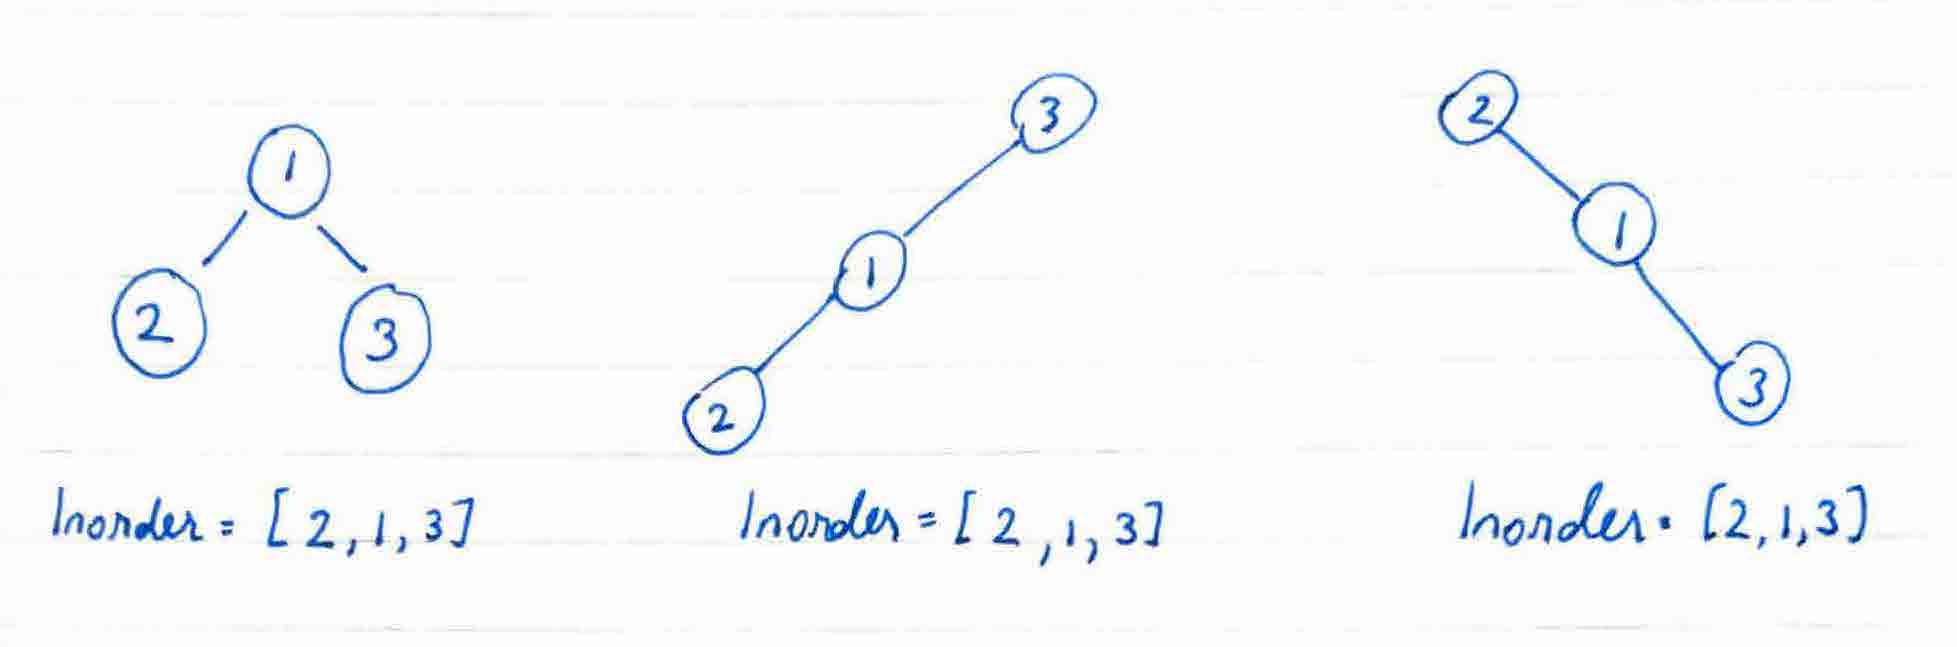
\includegraphics[width=14cm]{Inorder_wrong.jpg}
\end{center}

\section{The Binary Tree Signature}

Here we define a basic datatype for bintree:

\nwfilename{2015PH10813.nw}\nwbegincode{1}\sublabel{NW6NVqj-4XyAA2-1}\nwmargintag{{\nwtagstyle{}\subpageref{NW6NVqj-4XyAA2-1}}}\moddef{Node~{\nwtagstyle{}\subpageref{NW6NVqj-4XyAA2-1}}}\endmoddef\nwstartdeflinemarkup\nwusesondefline{\\{NW6NVqj-4WBYwn-1}\\{NW6NVqj-2nTQtw-1}}\nwenddeflinemarkup
        datatype 'a bintree = 
                Empty 
                | Node of 'a * 'a bintree * 'a bintree
\nwused{\\{NW6NVqj-4WBYwn-1}\\{NW6NVqj-2nTQtw-1}}\nwendcode{}\nwbegindocs{2}\nwdocspar

We also define a option datatype, since we intend to store the empty Leaf nodes as well

\nwenddocs{}\nwbegincode{3}\sublabel{NW6NVqj-4JPyOG-1}\nwmargintag{{\nwtagstyle{}\subpageref{NW6NVqj-4JPyOG-1}}}\moddef{Option~{\nwtagstyle{}\subpageref{NW6NVqj-4JPyOG-1}}}\endmoddef\nwstartdeflinemarkup\nwusesondefline{\\{NW6NVqj-4WBYwn-1}\\{NW6NVqj-2nTQtw-1}}\nwenddeflinemarkup
        datatype 'a option = NONE | SOME of 'a
\nwused{\\{NW6NVqj-4WBYwn-1}\\{NW6NVqj-2nTQtw-1}}\nwendcode{}\nwbegindocs{4}\nwdocspar

We define our regular preorder \& postorder functions like in the \href{http://www.cse.iitd.ernet.in/~sak/courses/ilfp/recover.pdf}{document}. Here \textbf{'a option list} implies a list which can contain \textbf{NONE} in case of Empty subtree or \textbf{SOME of value}

\nwenddocs{}\nwbegincode{5}\sublabel{NW6NVqj-azPlp-1}\nwmargintag{{\nwtagstyle{}\subpageref{NW6NVqj-azPlp-1}}}\moddef{PrePostSig~{\nwtagstyle{}\subpageref{NW6NVqj-azPlp-1}}}\endmoddef\nwstartdeflinemarkup\nwusesondefline{\\{NW6NVqj-4WBYwn-1}}\nwenddeflinemarkup
        val preorder : 'a bintree ->  'a option list
        val postorder : 'a bintree -> 'a option list
\nwused{\\{NW6NVqj-4WBYwn-1}}\nwendcode{}\nwbegindocs{6}\nwdocspar

However, for inorder, this is not enough. We need some addition \textit{Cosmetic Sugar} to gain the missing structural information in this traversal. Hence, we include the depth of a node defined to be 0 for the root node, and the depth of any child is 1 + the depth of their parent. \\
So, our node now contains a Tuple (value, depth) which is returned from the inorder traversal. Now we can define the signatures of the inorder and inorderInverse

\nwenddocs{}\nwbegincode{7}\sublabel{NW6NVqj-2NTUdd-1}\nwmargintag{{\nwtagstyle{}\subpageref{NW6NVqj-2NTUdd-1}}}\moddef{InSig~{\nwtagstyle{}\subpageref{NW6NVqj-2NTUdd-1}}}\endmoddef\nwstartdeflinemarkup\nwusesondefline{\\{NW6NVqj-4WBYwn-1}}\nwenddeflinemarkup
        val inorder : 'a bintree -> ('a option * int) list
        val inorderInverse : ('a option * int) list -> 'a bintree
\nwused{\\{NW6NVqj-4WBYwn-1}}\nwendcode{}\nwbegindocs{8}\nwdocspar

One last function we use to check if two given trees are equal. For this, we find their preorder and postorder traversals, and check their equality. 
\nwenddocs{}\nwbegincode{9}\sublabel{NW6NVqj-3QvoFw-1}\nwmargintag{{\nwtagstyle{}\subpageref{NW6NVqj-3QvoFw-1}}}\moddef{equalSig~{\nwtagstyle{}\subpageref{NW6NVqj-3QvoFw-1}}}\endmoddef\nwstartdeflinemarkup\nwusesondefline{\\{NW6NVqj-4WBYwn-1}}\nwenddeflinemarkup
        val checkTrees : ''a bintree * ''a bintree -> bool
\nwused{\\{NW6NVqj-4WBYwn-1}}\nwendcode{}\nwbegindocs{10}\nwdocspar

Now we can put everything together in our Signature

\nwenddocs{}\nwbegincode{11}\sublabel{NW6NVqj-4WBYwn-1}\nwmargintag{{\nwtagstyle{}\subpageref{NW6NVqj-4WBYwn-1}}}\moddef{bintreeSignature-complete~{\nwtagstyle{}\subpageref{NW6NVqj-4WBYwn-1}}}\endmoddef\nwstartdeflinemarkup\nwusesondefline{\\{NW6NVqj-2nTQtw-1}}\nwenddeflinemarkup
signature BINTREE = 
sig
\LA{}Node~{\nwtagstyle{}\subpageref{NW6NVqj-4XyAA2-1}}\RA{}
\LA{}Option~{\nwtagstyle{}\subpageref{NW6NVqj-4JPyOG-1}}\RA{}
        exception Empty_bintree;
        exception InvalidTraversal;
\LA{}PrePostSig~{\nwtagstyle{}\subpageref{NW6NVqj-azPlp-1}}\RA{}
\LA{}InSig~{\nwtagstyle{}\subpageref{NW6NVqj-2NTUdd-1}}\RA{}
\LA{}equalSig~{\nwtagstyle{}\subpageref{NW6NVqj-3QvoFw-1}}\RA{}
end
\nwused{\\{NW6NVqj-2nTQtw-1}}\nwendcode{}\nwbegindocs{12}\nwdocspar

\section{The Binary Tree Structure}

Similarly to the \href{http://www.cse.iitd.ernet.in/~sak/courses/ilfp/recover.pdf}{document} we define the preorder \& postorder functions using the tail recursive forms. \\

We use \textbf{NONE} to indicate empty nodes and \textbf{SOME of val}
to indicate nodes with value \textbf{val}
\nwenddocs{}\nwbegincode{13}\sublabel{NW6NVqj-FYIyT-1}\nwmargintag{{\nwtagstyle{}\subpageref{NW6NVqj-FYIyT-1}}}\moddef{preorder~{\nwtagstyle{}\subpageref{NW6NVqj-FYIyT-1}}}\endmoddef\nwstartdeflinemarkup\nwusesondefline{\\{NW6NVqj-2nTQtw-1}}\nwenddeflinemarkup
    local 
        fun pre(Empty, Llist) = NONE::Llist
                | pre(Node(N,Ltree, Rtree),Llist) = 
                let
                        val Mlist = pre(Rtree,Llist)
                        val Nlist = pre(Ltree,Mlist)
                in
                        SOME N :: Nlist
                end
        in 
                fun preorder T = pre(T,[])
        end
\nwused{\\{NW6NVqj-2nTQtw-1}}\nwendcode{}\nwbegindocs{14}\nwdocspar

\nwenddocs{}\nwbegincode{15}\sublabel{NW6NVqj-2drSLa-1}\nwmargintag{{\nwtagstyle{}\subpageref{NW6NVqj-2drSLa-1}}}\moddef{postorder~{\nwtagstyle{}\subpageref{NW6NVqj-2drSLa-1}}}\endmoddef\nwstartdeflinemarkup\nwusesondefline{\\{NW6NVqj-2nTQtw-1}}\nwenddeflinemarkup
    local 
        fun post(Empty, Llist) = NONE::Llist
                | post(Node(N,Ltree, Rtree),Llist) = 
                let
                        val Mlist = post(Rtree,SOME N::Llist)
                        val Nlist = post(Ltree,Mlist)
                in
                        Nlist
                end
        in 
                fun postorder T = post(T,[])
        end
\nwused{\\{NW6NVqj-2nTQtw-1}}\nwendcode{}\nwbegindocs{16}\nwdocspar

In inorder however, we need to store the depth of the node as well, since we are unable to figure out any strucural information from the traversal

\nwenddocs{}\nwbegincode{17}\sublabel{NW6NVqj-N7IVZ-1}\nwmargintag{{\nwtagstyle{}\subpageref{NW6NVqj-N7IVZ-1}}}\moddef{inorder~{\nwtagstyle{}\subpageref{NW6NVqj-N7IVZ-1}}}\endmoddef\nwstartdeflinemarkup\nwusesondefline{\\{NW6NVqj-2nTQtw-1}}\nwenddeflinemarkup
        local 
        fun ino(Empty, Llist,i) = (NONE,i)::Llist
                | ino(Node(N,Ltree, Rtree),Llist,i) = 
                let
                        val Mlist = ino(Rtree,Llist,i+1)
                        val Nlist = ino(Ltree,(SOME N,i)::Mlist,i+1)
                in
                        Nlist
                end
        in 
                fun inorder T = ino(T,[],0)
        end
\nwused{\\{NW6NVqj-2nTQtw-1}}\nwendcode{}\nwbegindocs{18}\nwdocspar

Here we store (value,depth) as a tuple in the node. \\

\subsection{The Inorder Inverse}

Before we start the inorder inverse function, we define some facts about our updated inorder Traversal (with heights)

\textit{\begin{enumerate}
    \item In any inorder traversal ($\bot$,\_) is the first and last element
    \item If any inorder traversal has more than 1 element, the tree is non-empty
    \item The descendants of a node always have a depth greater than the depth of the node. (\textbf{m},h1) \& (\textbf{n},h2) : n is a descendant of m if (h2 \textgreater h1)
    \item Any node m that has a height greater than a node l = (v,h) is either a descendant of l or a descendant of a sibling of l
    \item Any slice of the form [(\textbf{$\bot$},h+1), (\textbf{v},h), ($\neq \bot \neq$,h+1)] determines a unique leaf node in the tree with height h.
    \item Any slice of the form [(\textbf{$\bot$},h+2), (\textbf{m},h+1), (\textbf{$\bot$}, h+2), (\textbf{l},h), (\textbf{$\bot$},h+1)] where m $\neq \bot \neq$ l are values of the nodes, determines a unique subtree rooted at l whose left child is the leaf node m and the right child is empty
    \item Any slice of the form [(\textbf{$\bot$},h+1), (\textbf{l},h), (\textbf{$\bot$}, h+2), (\textbf{m},h+1), (\textbf{$\bot$},h+2)] where m $\neq \bot \neq$ l   are values of the nodes, determines a unique subtree rooted at l whose right
    child is the leaf node m and the left child is empty.
    \item Any slice of the form [(\textbf{T1},h+1), (\textbf{v},h), (\textbf{T2},h+1)] where T1  $\neq \bot \neq$ T2 are subtrees/leaf nodes determines a subtree rooted at v with T1 and T2 as it's left and right children
\end{enumerate}}

\textbf{Uniqueness of Inorder Traversal}: No two distinct binary trees can yield the same inorder traversal.
\textit{Proof:} The proof follows from the definition of inorder traversal and the previous facts (especially the if and only if
conditions) Further the statements yield an inductive proof along with a case analysis of the inductive step \\

Now we define some helper functions to create this inorder inverse. The first function converts a inorder traversal into a list of Bintree nodes. 

\nwenddocs{}\nwbegincode{19}\sublabel{NW6NVqj-3s4e0t-1}\nwmargintag{{\nwtagstyle{}\subpageref{NW6NVqj-3s4e0t-1}}}\moddef{Nodify~{\nwtagstyle{}\subpageref{NW6NVqj-3s4e0t-1}}}\endmoddef\nwstartdeflinemarkup\nwusesondefline{\\{NW6NVqj-D88LJ-1}}\nwenddeflinemarkup
    fun  Nodify[] = []
                | Nodify (h::t) = 
                Node(h,Empty,Empty)::Nodify(t)
\nwused{\\{NW6NVqj-D88LJ-1}}\nwendcode{}\nwbegindocs{20}\nwdocspar

The next function joins 3 nodes into a single node if the height of the middle node is one less than the other two.

\nwenddocs{}\nwbegincode{21}\sublabel{NW6NVqj-4eyur2-1}\nwmargintag{{\nwtagstyle{}\subpageref{NW6NVqj-4eyur2-1}}}\moddef{joinNodes~{\nwtagstyle{}\subpageref{NW6NVqj-4eyur2-1}}}\endmoddef\nwstartdeflinemarkup\nwusesondefline{\\{NW6NVqj-D88LJ-1}}\nwenddeflinemarkup
                fun joinNodes(T1 as Node((v1,h1),_,_), T2 as Node((v2,h2),_,_), T3 as Node((v3,h3),_,_)) =
                if(h1=h3 andalso (h1-1)=h2) then
                        [Node((v2,h2),T1,T3)]
                else
                        [T1,T2,T3]
                | joinNodes(T1,T2,T3) = raise InvalidTraversal
\nwused{\\{NW6NVqj-D88LJ-1}}\nwendcode{}\nwbegindocs{22}\nwdocspar

The next function goes over a list of notes and tries combining all the successive nodes triplets

\nwenddocs{}\nwbegincode{23}\sublabel{NW6NVqj-2W3UBo-1}\nwmargintag{{\nwtagstyle{}\subpageref{NW6NVqj-2W3UBo-1}}}\moddef{CombineIter~{\nwtagstyle{}\subpageref{NW6NVqj-2W3UBo-1}}}\endmoddef\nwstartdeflinemarkup\nwusesondefline{\\{NW6NVqj-D88LJ-1}}\nwenddeflinemarkup
        fun combineIter(h1::h2::h3::[]) = 
                        joinNodes(h1,h2,h3)
                | combineIter(L as h1::h2::h3::tl) = 
                let
                        val M = joinNodes(h1,h2,h3) @ tl
                in
                        List.hd(M) :: combineIter(List.tl(M))
                end
                | combineIter (L as h1::h2::[]) = L
                | combineIter L = raise InvalidTraversal
\nwused{\\{NW6NVqj-D88LJ-1}}\nwendcode{}\nwbegindocs{24}\nwdocspar

Now, a function keeps calling the iterative joining function until only one node remains

\nwenddocs{}\nwbegincode{25}\sublabel{NW6NVqj-3BQdfV-1}\nwmargintag{{\nwtagstyle{}\subpageref{NW6NVqj-3BQdfV-1}}}\moddef{Combine~{\nwtagstyle{}\subpageref{NW6NVqj-3BQdfV-1}}}\endmoddef\nwstartdeflinemarkup\nwusesondefline{\\{NW6NVqj-D88LJ-1}}\nwenddeflinemarkup
                fun combine(hd::[]) = hd
                | combine L =  
                let
                        val M = combineIter L
                in
                        combine M
                end
\nwused{\\{NW6NVqj-D88LJ-1}}\nwendcode{}\nwbegindocs{26}\nwdocspar

This tree created has Complete nodes even for Empty Leaf nodes. We need to clean this up and remove the extra Empty Nodes

\nwenddocs{}\nwbegincode{27}\sublabel{NW6NVqj-8c9SM-1}\nwmargintag{{\nwtagstyle{}\subpageref{NW6NVqj-8c9SM-1}}}\moddef{treeClean~{\nwtagstyle{}\subpageref{NW6NVqj-8c9SM-1}}}\endmoddef\nwstartdeflinemarkup\nwusesondefline{\\{NW6NVqj-D88LJ-1}}\nwenddeflinemarkup
                fun treeClean(Node((SOME v,_),Ltree,Rtree)) = 
                let
                        val LClean = treeClean(Ltree)
                        val RClean = treeClean(Rtree)
                in
                        Node(v, LClean, RClean)
                end
                | treeClean(T) = Empty
\nwused{\\{NW6NVqj-D88LJ-1}}\nwendcode{}\nwbegindocs{28}\nwdocspar

Now we can put it all together in our inorderInverse

\nwenddocs{}\nwbegincode{29}\sublabel{NW6NVqj-D88LJ-1}\nwmargintag{{\nwtagstyle{}\subpageref{NW6NVqj-D88LJ-1}}}\moddef{inorderInverse~{\nwtagstyle{}\subpageref{NW6NVqj-D88LJ-1}}}\endmoddef\nwstartdeflinemarkup\nwusesondefline{\\{NW6NVqj-2nTQtw-1}}\nwenddeflinemarkup
    local
        \LA{}Nodify~{\nwtagstyle{}\subpageref{NW6NVqj-3s4e0t-1}}\RA{}
        \LA{}joinNodes~{\nwtagstyle{}\subpageref{NW6NVqj-4eyur2-1}}\RA{}
        \LA{}CombineIter~{\nwtagstyle{}\subpageref{NW6NVqj-2W3UBo-1}}\RA{}
        \LA{}Combine~{\nwtagstyle{}\subpageref{NW6NVqj-3BQdfV-1}}\RA{}
        \LA{}treeClean~{\nwtagstyle{}\subpageref{NW6NVqj-8c9SM-1}}\RA{}
    in
        fun inorderInverse(L) = 
                        treeClean (combine (Nodify L))

        end
\nwused{\\{NW6NVqj-2nTQtw-1}}\nwendcode{}\nwbegindocs{30}\nwdocspar

Having gotten a tree back from an inorder inverse, we would like to define a function to check if the tree is the same as our original tree. We can do the same by comparing their preorder \& postorder traversal. (Since in the \href{http://www.cse.iitd.ernet.in/~sak/courses/ilfp/recover.pdf}{document} the uniqueness of preorder/postorder traversals has been proved. For this we need to check if two lists generated by the traversals are the same

\nwenddocs{}\nwbegincode{31}\sublabel{NW6NVqj-2cpULM-1}\nwmargintag{{\nwtagstyle{}\subpageref{NW6NVqj-2cpULM-1}}}\moddef{checkList~{\nwtagstyle{}\subpageref{NW6NVqj-2cpULM-1}}}\endmoddef\nwstartdeflinemarkup\nwusesondefline{\\{NW6NVqj-1Uzkdr-1}}\nwenddeflinemarkup
    fun checkList([],[]) = true
                | checkList([],_) = false
                | checkList(_,[]) = false
                | checkList(NONE::t1, NONE::t2) = checkList(t1,t2)
                | checkList(SOME h1::t1, SOME h2::t2) = 
                if(h1=h2) then
                        checkList(t1,t2)
                else
                        false
                | checkList(_,_) = false
\nwused{\\{NW6NVqj-1Uzkdr-1}}\nwendcode{}\nwbegindocs{32}\nwdocspar

\nwenddocs{}\nwbegincode{33}\sublabel{NW6NVqj-1Uzkdr-1}\nwmargintag{{\nwtagstyle{}\subpageref{NW6NVqj-1Uzkdr-1}}}\moddef{checkTrees~{\nwtagstyle{}\subpageref{NW6NVqj-1Uzkdr-1}}}\endmoddef\nwstartdeflinemarkup\nwusesondefline{\\{NW6NVqj-2nTQtw-1}}\nwenddeflinemarkup
    local
                \LA{}checkList~{\nwtagstyle{}\subpageref{NW6NVqj-2cpULM-1}}\RA{}
        in
                fun checkTrees(T1,T2) = 
                let
                        val pre1 = preorder(T1)
                        val pre2 = preorder(T2)
                        val pos1 = postorder(T1)
                        val pos2 = postorder(T2)
                in
                        if(checkList(pre1,pre2) andalso checkList(pos1,pos2)) then
                                true
                        else
                                false
                end
        end
\nwused{\\{NW6NVqj-2nTQtw-1}}\nwendcode{}\nwbegindocs{34}\nwdocspar

Now we put it all together into our Bintree structure

\nwenddocs{}\nwbegincode{35}\sublabel{NW6NVqj-2nTQtw-1}\nwmargintag{{\nwtagstyle{}\subpageref{NW6NVqj-2nTQtw-1}}}\moddef{bintreeStructure-complete~{\nwtagstyle{}\subpageref{NW6NVqj-2nTQtw-1}}}\endmoddef\nwstartdeflinemarkup\nwusesondefline{\\{NW6NVqj-stHGb-1}}\nwenddeflinemarkup
\LA{}bintreeSignature-complete~{\nwtagstyle{}\subpageref{NW6NVqj-4WBYwn-1}}\RA{}
structure Bintree : BINTREE = 
struct
    \LA{}Node~{\nwtagstyle{}\subpageref{NW6NVqj-4XyAA2-1}}\RA{}
    \LA{}Option~{\nwtagstyle{}\subpageref{NW6NVqj-4JPyOG-1}}\RA{}
    
    exception Empty_bintree
        exception InvalidTraversal
        
        \LA{}preorder~{\nwtagstyle{}\subpageref{NW6NVqj-FYIyT-1}}\RA{}
        \LA{}postorder~{\nwtagstyle{}\subpageref{NW6NVqj-2drSLa-1}}\RA{}
        \LA{}inorder~{\nwtagstyle{}\subpageref{NW6NVqj-N7IVZ-1}}\RA{}
    \LA{}inorderInverse~{\nwtagstyle{}\subpageref{NW6NVqj-D88LJ-1}}\RA{}
    \LA{}checkTrees~{\nwtagstyle{}\subpageref{NW6NVqj-1Uzkdr-1}}\RA{}
end
\nwused{\\{NW6NVqj-stHGb-1}}\nwendcode{}\nwbegindocs{36}\nwdocspar

\section{Test Cases}

We define the following test cases to check the performance of our inorderInverse 

\begin{center}
        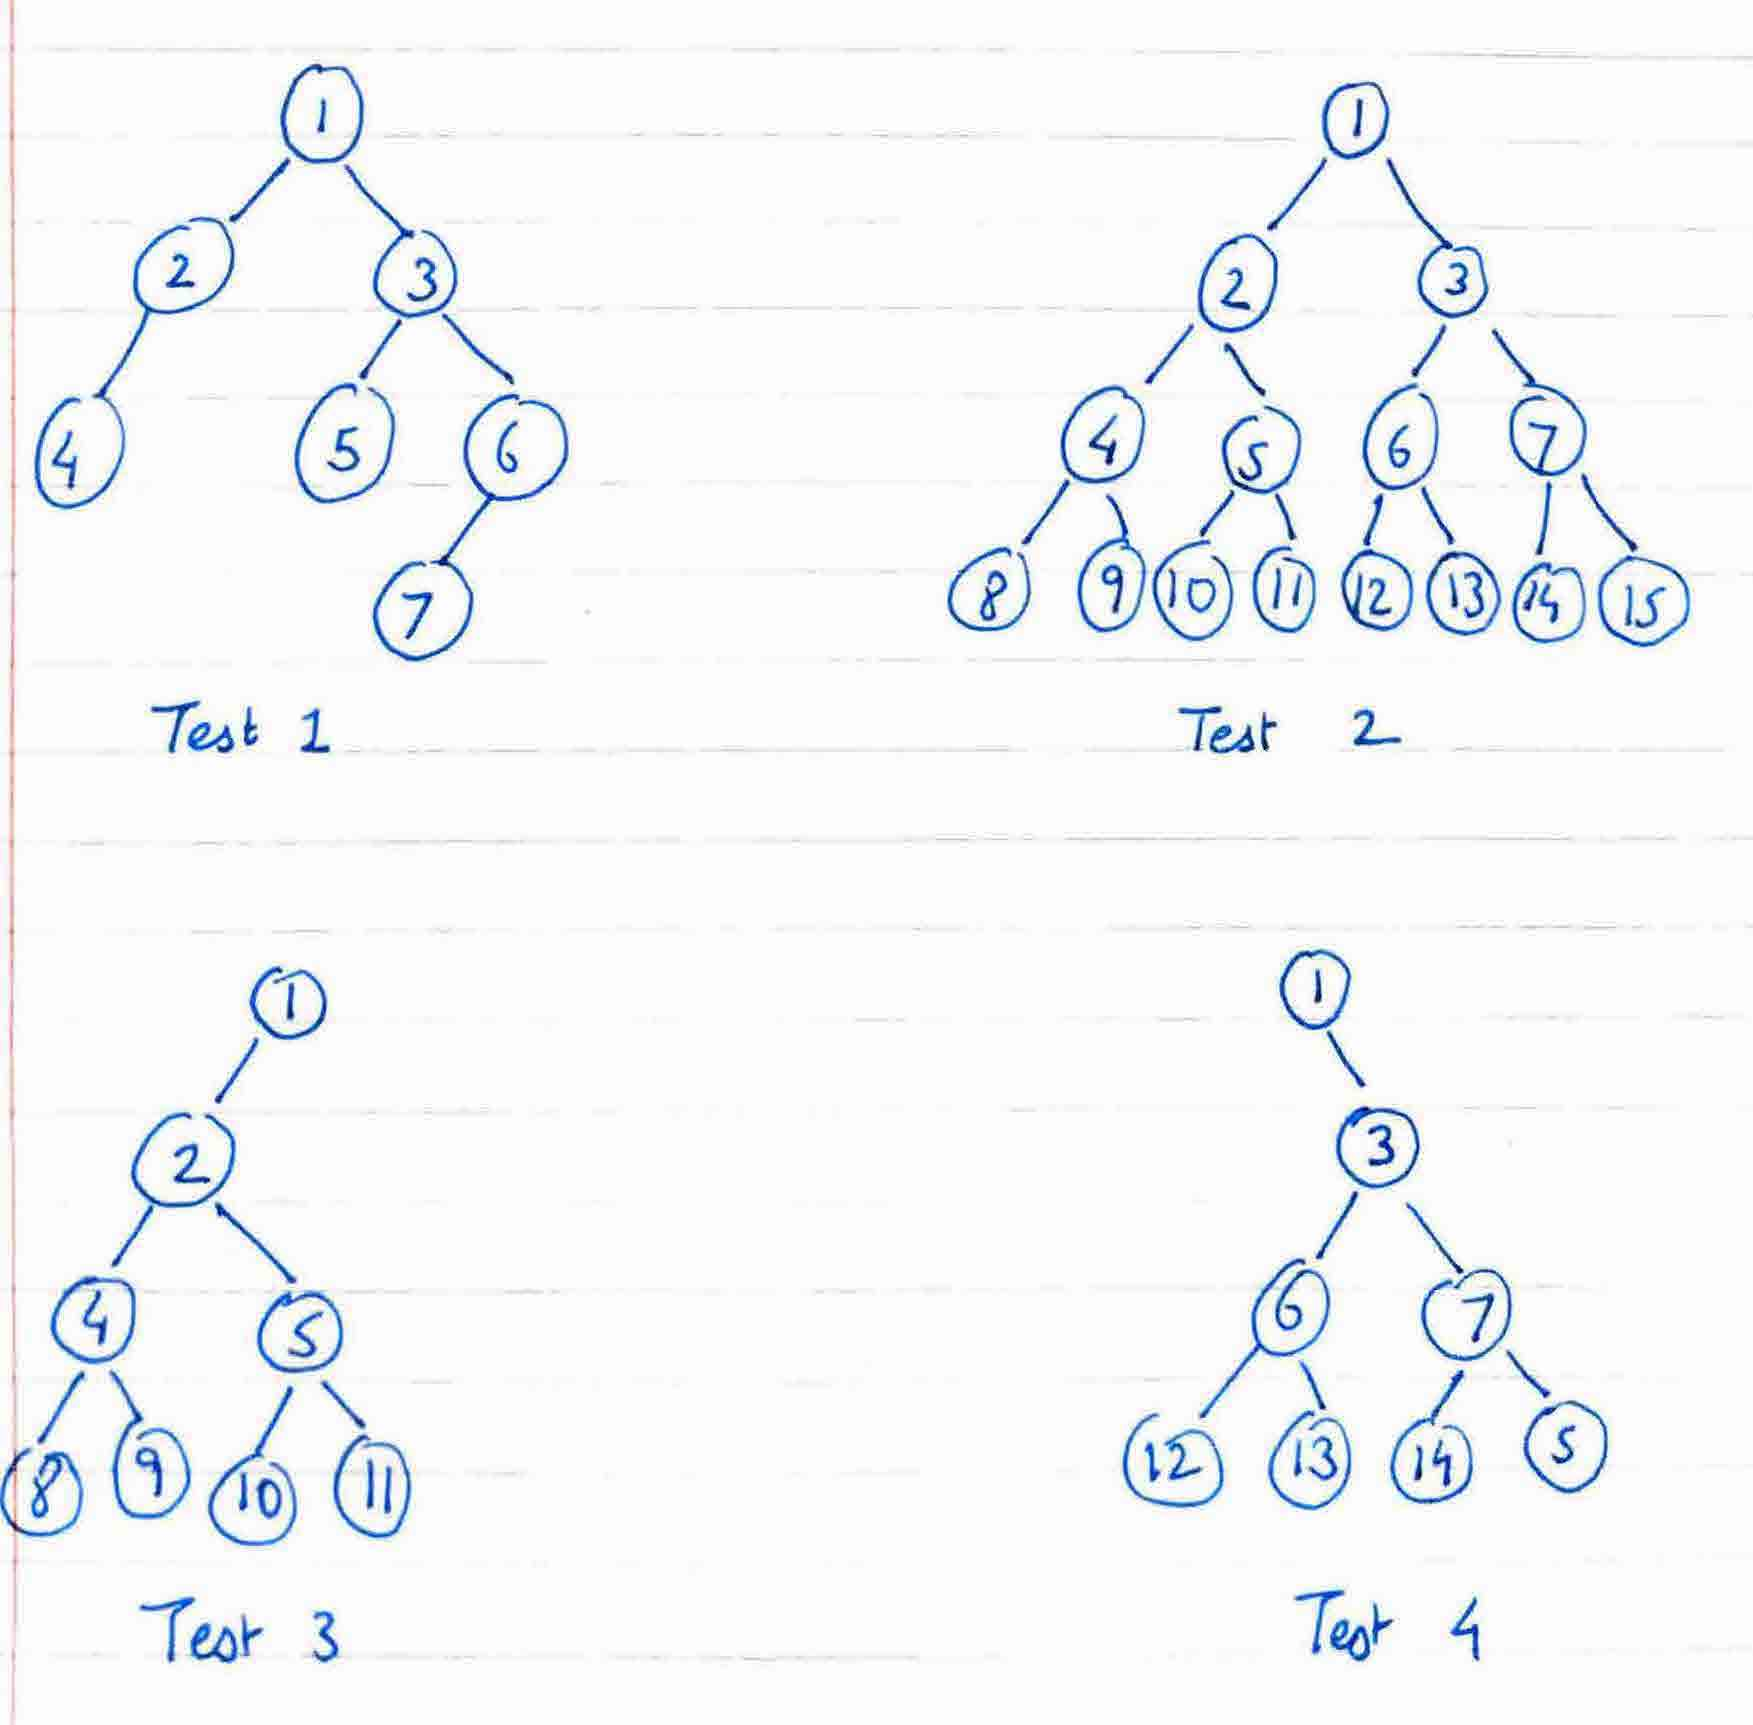
\includegraphics[width=14cm]{Test1.jpg}
        \\
        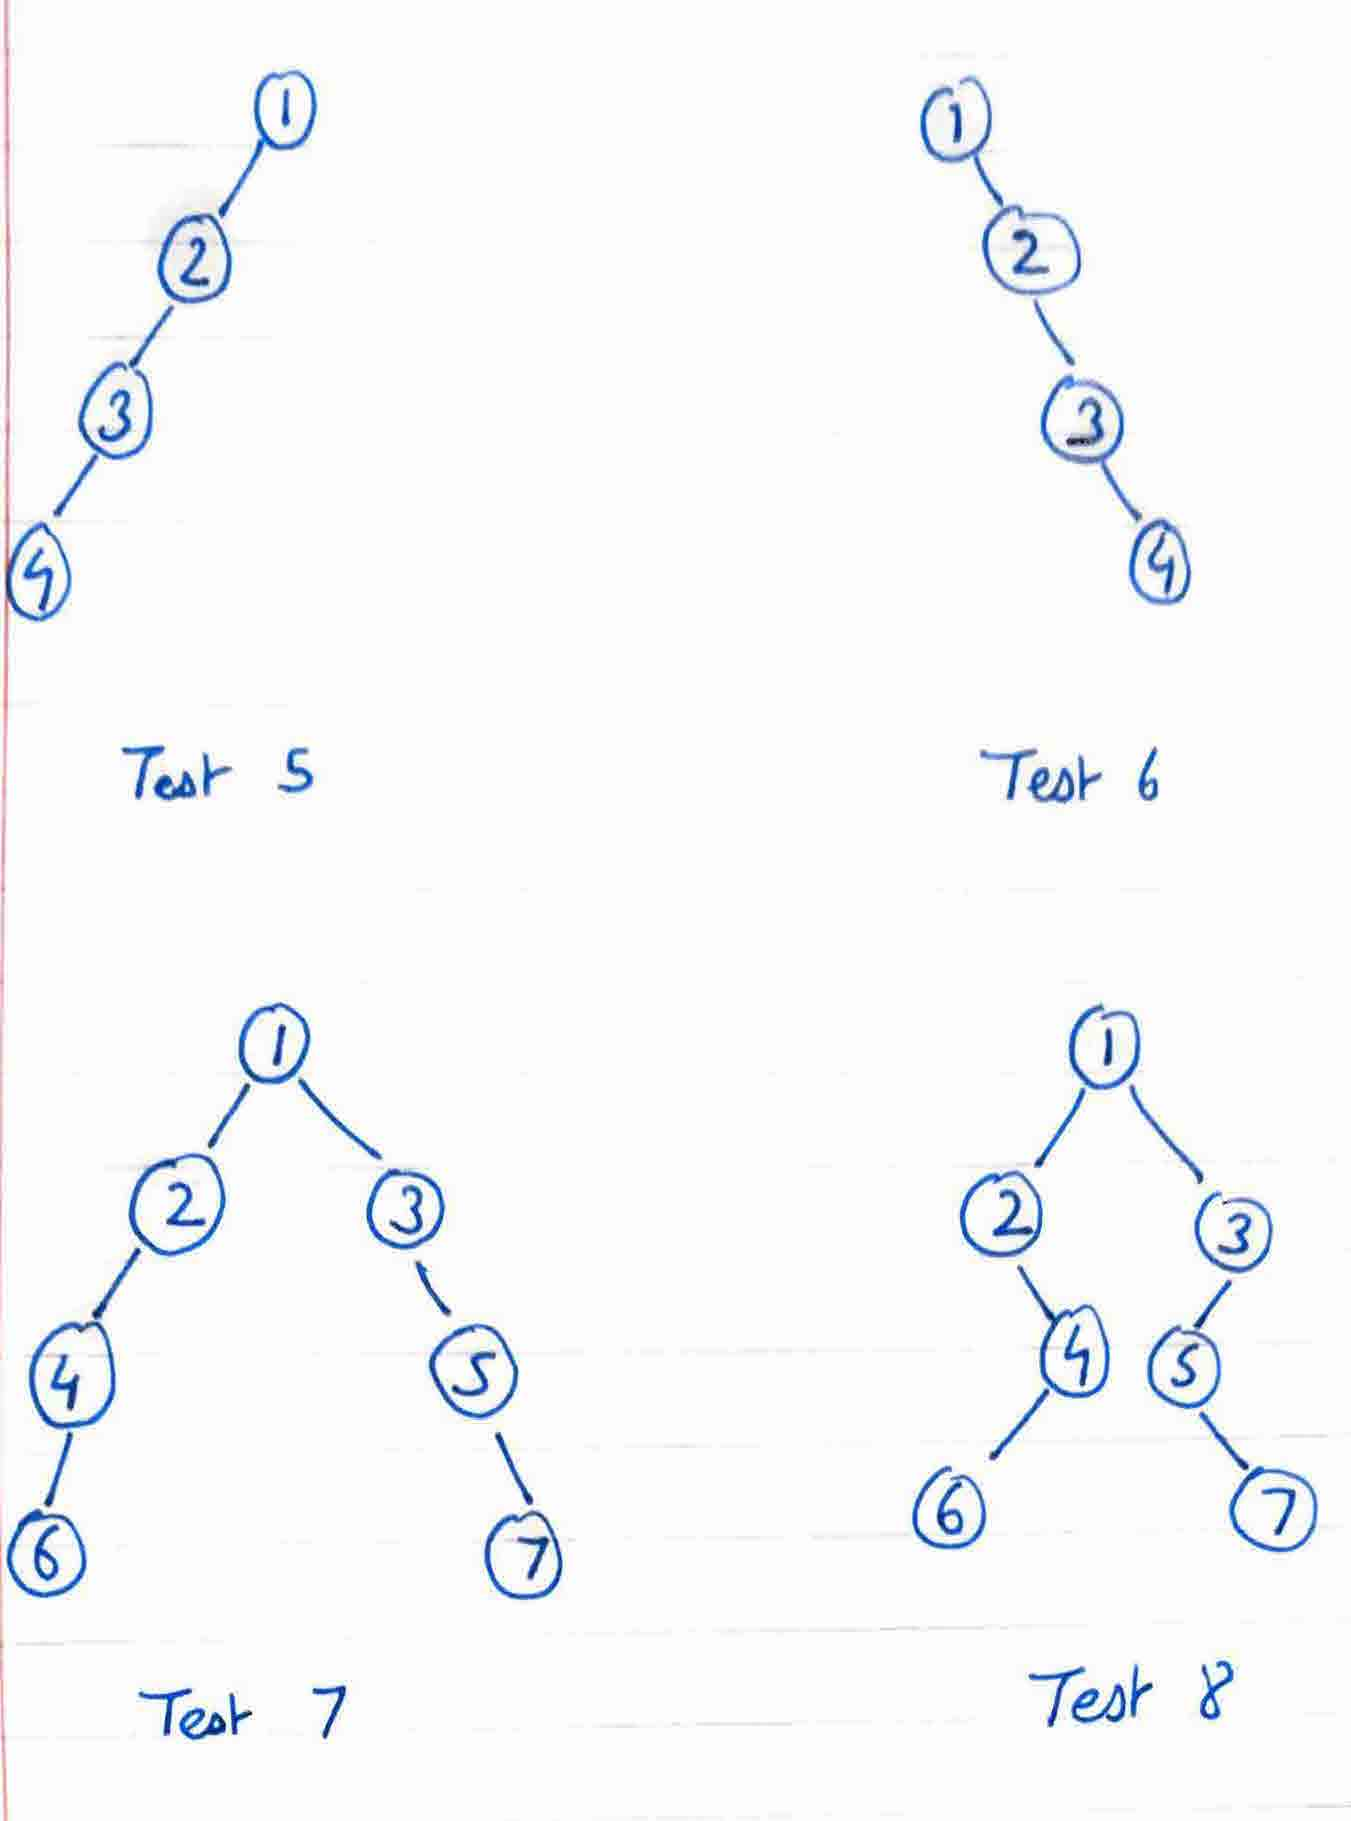
\includegraphics[width=14cm]{Test2.jpg}
\end{center}
\nwenddocs{}\nwbegincode{37}\sublabel{NW6NVqj-2obuBU-1}\nwmargintag{{\nwtagstyle{}\subpageref{NW6NVqj-2obuBU-1}}}\moddef{test1~{\nwtagstyle{}\subpageref{NW6NVqj-2obuBU-1}}}\endmoddef\nwstartdeflinemarkup\nwusesondefline{\\{NW6NVqj-stHGb-1}}\nwenddeflinemarkup
local
        val t7 = Node (7, Empty, Empty);
        val t6 = Node (6, t7, Empty);
        val t5 = Node (5, Empty, Empty);
        val t4 = Node (4, Empty, Empty);
        val t3 = Node (3, t5, t6);
        val t2 = Node (2, Empty, t4);
in
        val test1 = Node (1, t2, t3);
end
\nwused{\\{NW6NVqj-stHGb-1}}\nwendcode{}\nwbegindocs{38}\nwdocspar
\nwenddocs{}\nwbegincode{39}\sublabel{NW6NVqj-PItlY-1}\nwmargintag{{\nwtagstyle{}\subpageref{NW6NVqj-PItlY-1}}}\moddef{test2~{\nwtagstyle{}\subpageref{NW6NVqj-PItlY-1}}}\endmoddef\nwstartdeflinemarkup\nwusesondefline{\\{NW6NVqj-stHGb-1}}\nwenddeflinemarkup
local
        val t15 = Node (15, Empty, Empty);
        val t14 = Node (14, Empty, Empty);
        val t13 = Node (13, Empty, Empty);
        val t12 = Node (12, Empty, Empty);
        val t11 = Node (11, Empty, Empty);
        val t10 = Node (10, Empty, Empty);
        val t9 = Node (9, Empty, Empty);
        val t8 = Node (8, Empty, Empty);
        val t7 = Node(7, t14, t15);
        val t6 = Node (6, t12, t13);
        val t5 = Node (5, t10, t11);
        val t4 = Node (4, t8, t9);
        val t3 = Node (3, t6, t7);
        val t2 = Node (2, t4, t5);
in
        val test2 = Node (1, t2, t3);
end
\nwused{\\{NW6NVqj-stHGb-1}}\nwendcode{}\nwbegindocs{40}\nwdocspar
\nwenddocs{}\nwbegincode{41}\sublabel{NW6NVqj-4A3yQS-1}\nwmargintag{{\nwtagstyle{}\subpageref{NW6NVqj-4A3yQS-1}}}\moddef{test3~{\nwtagstyle{}\subpageref{NW6NVqj-4A3yQS-1}}}\endmoddef\nwstartdeflinemarkup\nwusesondefline{\\{NW6NVqj-stHGb-1}}\nwenddeflinemarkup
local
        val t11 = Node (11, Empty, Empty);
        val t10 = Node (10, Empty, Empty);
        val t9 = Node (9, Empty, Empty);
        val t8 = Node (8, Empty, Empty);
        val t5 = Node (5, t10, t11);
        val t4 = Node (4, t8, t9);
        val t2 = Node (2, t4, t5);
in
        val test3 = Node (1, t2, Empty);
end

\nwused{\\{NW6NVqj-stHGb-1}}\nwendcode{}\nwbegincode{42}\sublabel{NW6NVqj-1UZpaq-1}\nwmargintag{{\nwtagstyle{}\subpageref{NW6NVqj-1UZpaq-1}}}\moddef{test4~{\nwtagstyle{}\subpageref{NW6NVqj-1UZpaq-1}}}\endmoddef\nwstartdeflinemarkup\nwusesondefline{\\{NW6NVqj-stHGb-1}}\nwenddeflinemarkup
local
        val t15 = Node (15, Empty, Empty);
        val t14 = Node (14, Empty, Empty);
        val t13 = Node (13, Empty, Empty);
        val t12 = Node (12, Empty, Empty);
        val t7 = Node(7, t14, t15);
        val t6 = Node (6, t12, t13);
        val t3 = Node (3, t6, t7);
in
        val test4 = Node (1, Empty, t3);
end
\nwused{\\{NW6NVqj-stHGb-1}}\nwendcode{}\nwbegindocs{43}\nwdocspar
\nwenddocs{}\nwbegincode{44}\sublabel{NW6NVqj-30oemG-1}\nwmargintag{{\nwtagstyle{}\subpageref{NW6NVqj-30oemG-1}}}\moddef{test5~{\nwtagstyle{}\subpageref{NW6NVqj-30oemG-1}}}\endmoddef\nwstartdeflinemarkup\nwusesondefline{\\{NW6NVqj-stHGb-1}}\nwenddeflinemarkup
local
        val t4 = Node (4, Empty, Empty);
        val t3 = Node (3, t4, Empty);
        val t2 = Node (2, t3, Empty);
in
        val test5 = Node (1, t2, Empty);
end

\nwused{\\{NW6NVqj-stHGb-1}}\nwendcode{}\nwbegincode{45}\sublabel{NW6NVqj-mrbYu-1}\nwmargintag{{\nwtagstyle{}\subpageref{NW6NVqj-mrbYu-1}}}\moddef{test6~{\nwtagstyle{}\subpageref{NW6NVqj-mrbYu-1}}}\endmoddef\nwstartdeflinemarkup\nwusesondefline{\\{NW6NVqj-stHGb-1}}\nwenddeflinemarkup
local
        val t4 = Node (4, Empty, Empty);
        val t3 = Node (3, Empty, t4);
        val t2 = Node (2, Empty, t3);
in
        val test6 = Node (1, Empty, t2);
end
\nwused{\\{NW6NVqj-stHGb-1}}\nwendcode{}\nwbegindocs{46}\nwdocspar
\nwenddocs{}\nwbegincode{47}\sublabel{NW6NVqj-446Oh6-1}\nwmargintag{{\nwtagstyle{}\subpageref{NW6NVqj-446Oh6-1}}}\moddef{test7~{\nwtagstyle{}\subpageref{NW6NVqj-446Oh6-1}}}\endmoddef\nwstartdeflinemarkup\nwusesondefline{\\{NW6NVqj-stHGb-1}}\nwenddeflinemarkup
local
        val t7 = Node (7, Empty, Empty);
        val t6 = Node (6, Empty, Empty);
        val t5 = Node (5, Empty, t7);
        val t4 = Node (4, t6, Empty);
        val t3 = Node (3, Empty, t5);
        val t2 = Node (2, t4, Empty);
in
        val test7 = Node (1, t2, t3);
end
\nwused{\\{NW6NVqj-stHGb-1}}\nwendcode{}\nwbegindocs{48}\nwdocspar
\nwenddocs{}\nwbegincode{49}\sublabel{NW6NVqj-25u5CK-1}\nwmargintag{{\nwtagstyle{}\subpageref{NW6NVqj-25u5CK-1}}}\moddef{test8~{\nwtagstyle{}\subpageref{NW6NVqj-25u5CK-1}}}\endmoddef\nwstartdeflinemarkup\nwusesondefline{\\{NW6NVqj-stHGb-1}}\nwenddeflinemarkup
local
        val t7 = Node (7, Empty, Empty);
        val t6 = Node (6, Empty, Empty);
        val t5 = Node (5, Empty, t7);
        val t4 = Node (4, t6, Empty);
        val t3 = Node (3, t5, Empty);
        val t2 = Node (2, Empty, t4);
in
        val test8 = Node (1, t2, t3);
end
\nwused{\\{NW6NVqj-stHGb-1}}\nwendcode{}\nwbegindocs{50}\nwdocspar

After this, to check if our inorderInverse works for each test case, we simply checkTrees between the inorderInverse generated tree and the original tree

\nwenddocs{}\nwbegincode{51}\sublabel{NW6NVqj-2UuN4Q-1}\nwmargintag{{\nwtagstyle{}\subpageref{NW6NVqj-2UuN4Q-1}}}\moddef{testCheck~{\nwtagstyle{}\subpageref{NW6NVqj-2UuN4Q-1}}}\endmoddef\nwstartdeflinemarkup\nwusesondefline{\\{NW6NVqj-stHGb-1}}\nwenddeflinemarkup
val test1_check = checkTrees(inorderInverse(inorder(test1)),test1);
val test2_check = checkTrees(inorderInverse(inorder(test2)),test2);
val test3_check = checkTrees(inorderInverse(inorder(test3)),test3);
val test4_check = checkTrees(inorderInverse(inorder(test4)),test4);
val test5_check = checkTrees(inorderInverse(inorder(test5)),test5);
val test6_check = checkTrees(inorderInverse(inorder(test6)),test6);
val test7_check = checkTrees(inorderInverse(inorder(test7)),test7);
val test8_check = checkTrees(inorderInverse(inorder(test8)),test8);
\nwused{\\{NW6NVqj-stHGb-1}}\nwendcode{}\nwbegindocs{52}\nwdocspar

\nwenddocs{}\nwbegincode{53}\sublabel{NW6NVqj-stHGb-1}\nwmargintag{{\nwtagstyle{}\subpageref{NW6NVqj-stHGb-1}}}\moddef{testCase-complete~{\nwtagstyle{}\subpageref{NW6NVqj-stHGb-1}}}\endmoddef\nwstartdeflinemarkup\nwenddeflinemarkup
\LA{}bintreeStructure-complete~{\nwtagstyle{}\subpageref{NW6NVqj-2nTQtw-1}}\RA{}
open Bintree;

\LA{}test1~{\nwtagstyle{}\subpageref{NW6NVqj-2obuBU-1}}\RA{}
\LA{}test2~{\nwtagstyle{}\subpageref{NW6NVqj-PItlY-1}}\RA{}
\LA{}test3~{\nwtagstyle{}\subpageref{NW6NVqj-4A3yQS-1}}\RA{}
\LA{}test4~{\nwtagstyle{}\subpageref{NW6NVqj-1UZpaq-1}}\RA{}
\LA{}test5~{\nwtagstyle{}\subpageref{NW6NVqj-30oemG-1}}\RA{}
\LA{}test6~{\nwtagstyle{}\subpageref{NW6NVqj-mrbYu-1}}\RA{}
\LA{}test7~{\nwtagstyle{}\subpageref{NW6NVqj-446Oh6-1}}\RA{}
\LA{}test8~{\nwtagstyle{}\subpageref{NW6NVqj-25u5CK-1}}\RA{}
\LA{}testCheck~{\nwtagstyle{}\subpageref{NW6NVqj-2UuN4Q-1}}\RA{}
\nwnotused{testCase-complete}\nwendcode{}

\nwixlogsorted{c}{{bintreeSignature-complete}{NW6NVqj-4WBYwn-1}{\nwixd{NW6NVqj-4WBYwn-1}\nwixu{NW6NVqj-2nTQtw-1}}}%
\nwixlogsorted{c}{{bintreeStructure-complete}{NW6NVqj-2nTQtw-1}{\nwixd{NW6NVqj-2nTQtw-1}\nwixu{NW6NVqj-stHGb-1}}}%
\nwixlogsorted{c}{{checkList}{NW6NVqj-2cpULM-1}{\nwixd{NW6NVqj-2cpULM-1}\nwixu{NW6NVqj-1Uzkdr-1}}}%
\nwixlogsorted{c}{{checkTrees}{NW6NVqj-1Uzkdr-1}{\nwixd{NW6NVqj-1Uzkdr-1}\nwixu{NW6NVqj-2nTQtw-1}}}%
\nwixlogsorted{c}{{Combine}{NW6NVqj-3BQdfV-1}{\nwixd{NW6NVqj-3BQdfV-1}\nwixu{NW6NVqj-D88LJ-1}}}%
\nwixlogsorted{c}{{CombineIter}{NW6NVqj-2W3UBo-1}{\nwixd{NW6NVqj-2W3UBo-1}\nwixu{NW6NVqj-D88LJ-1}}}%
\nwixlogsorted{c}{{equalSig}{NW6NVqj-3QvoFw-1}{\nwixd{NW6NVqj-3QvoFw-1}\nwixu{NW6NVqj-4WBYwn-1}}}%
\nwixlogsorted{c}{{inorder}{NW6NVqj-N7IVZ-1}{\nwixd{NW6NVqj-N7IVZ-1}\nwixu{NW6NVqj-2nTQtw-1}}}%
\nwixlogsorted{c}{{inorderInverse}{NW6NVqj-D88LJ-1}{\nwixd{NW6NVqj-D88LJ-1}\nwixu{NW6NVqj-2nTQtw-1}}}%
\nwixlogsorted{c}{{InSig}{NW6NVqj-2NTUdd-1}{\nwixd{NW6NVqj-2NTUdd-1}\nwixu{NW6NVqj-4WBYwn-1}}}%
\nwixlogsorted{c}{{joinNodes}{NW6NVqj-4eyur2-1}{\nwixd{NW6NVqj-4eyur2-1}\nwixu{NW6NVqj-D88LJ-1}}}%
\nwixlogsorted{c}{{Node}{NW6NVqj-4XyAA2-1}{\nwixd{NW6NVqj-4XyAA2-1}\nwixu{NW6NVqj-4WBYwn-1}\nwixu{NW6NVqj-2nTQtw-1}}}%
\nwixlogsorted{c}{{Nodify}{NW6NVqj-3s4e0t-1}{\nwixd{NW6NVqj-3s4e0t-1}\nwixu{NW6NVqj-D88LJ-1}}}%
\nwixlogsorted{c}{{Option}{NW6NVqj-4JPyOG-1}{\nwixd{NW6NVqj-4JPyOG-1}\nwixu{NW6NVqj-4WBYwn-1}\nwixu{NW6NVqj-2nTQtw-1}}}%
\nwixlogsorted{c}{{postorder}{NW6NVqj-2drSLa-1}{\nwixd{NW6NVqj-2drSLa-1}\nwixu{NW6NVqj-2nTQtw-1}}}%
\nwixlogsorted{c}{{preorder}{NW6NVqj-FYIyT-1}{\nwixd{NW6NVqj-FYIyT-1}\nwixu{NW6NVqj-2nTQtw-1}}}%
\nwixlogsorted{c}{{PrePostSig}{NW6NVqj-azPlp-1}{\nwixd{NW6NVqj-azPlp-1}\nwixu{NW6NVqj-4WBYwn-1}}}%
\nwixlogsorted{c}{{test1}{NW6NVqj-2obuBU-1}{\nwixd{NW6NVqj-2obuBU-1}\nwixu{NW6NVqj-stHGb-1}}}%
\nwixlogsorted{c}{{test2}{NW6NVqj-PItlY-1}{\nwixd{NW6NVqj-PItlY-1}\nwixu{NW6NVqj-stHGb-1}}}%
\nwixlogsorted{c}{{test3}{NW6NVqj-4A3yQS-1}{\nwixd{NW6NVqj-4A3yQS-1}\nwixu{NW6NVqj-stHGb-1}}}%
\nwixlogsorted{c}{{test4}{NW6NVqj-1UZpaq-1}{\nwixd{NW6NVqj-1UZpaq-1}\nwixu{NW6NVqj-stHGb-1}}}%
\nwixlogsorted{c}{{test5}{NW6NVqj-30oemG-1}{\nwixd{NW6NVqj-30oemG-1}\nwixu{NW6NVqj-stHGb-1}}}%
\nwixlogsorted{c}{{test6}{NW6NVqj-mrbYu-1}{\nwixd{NW6NVqj-mrbYu-1}\nwixu{NW6NVqj-stHGb-1}}}%
\nwixlogsorted{c}{{test7}{NW6NVqj-446Oh6-1}{\nwixd{NW6NVqj-446Oh6-1}\nwixu{NW6NVqj-stHGb-1}}}%
\nwixlogsorted{c}{{test8}{NW6NVqj-25u5CK-1}{\nwixd{NW6NVqj-25u5CK-1}\nwixu{NW6NVqj-stHGb-1}}}%
\nwixlogsorted{c}{{testCase-complete}{NW6NVqj-stHGb-1}{\nwixd{NW6NVqj-stHGb-1}}}%
\nwixlogsorted{c}{{testCheck}{NW6NVqj-2UuN4Q-1}{\nwixd{NW6NVqj-2UuN4Q-1}\nwixu{NW6NVqj-stHGb-1}}}%
\nwixlogsorted{c}{{treeClean}{NW6NVqj-8c9SM-1}{\nwixd{NW6NVqj-8c9SM-1}\nwixu{NW6NVqj-D88LJ-1}}}%
\nwbegindocs{54}\nwdocspar

The reason to choose these particular test cases since it covers some particular ambiguous cases such as a fully dense tree (Test2), a highly skewed tree (Test5 and Test6) as well as a initially skewed and then dense tree (Test3 and Test4) or a highly hollow tree (Test7) as well as a tree containing alternative oriented children (Test8)

The checkTrees function checks the inorderInverse generated tree vs the original tree. For all these testcases, the output is true.

\end{document}
\nwenddocs{}
